%Iniciação de pacotes e linguagens
\documentclass[12pt]{article}
\usepackage{fatec-ti}
\usepackage{url}
\def\UrlBreaks{\do\/\do-}
\usepackage{graphicx,url}
\usepackage[brazil]{babel}
\usepackage[utf8]{inputenc}
\usepackage{longtable}
\usepackage{tabularx}
\usepackage{float}
\usepackage{tikz}
\usetikzlibrary{positioning,arrows.meta,shapes.geometric}
\sloppy

%Título do TCC
\title{Nexus: uma Plataforma Unificada de Gestão de Projetos, Documentação e Comunicação para Equipes de Desenvolvimento de Software\\ Trabalho de Conclusão de Curso 2}

\author{Pedro Gentil Roodes Rodrigues\inst{1}, Angelo Gonçalves da Luz\inst{1}}

\address{Curso de Análise e Desenvolvimento de Sistemas -- Faculdade de Tecnologia SENAC Pelotas\\
  Rua Gonçalves Chaves 602 -- 96015560 -- Pelotas -- RS -- Brazil
  \email{pedro.rodrigues@aluno.senacrs.edu.br}
}

\begin{document}

\maketitle

\begin{abstract}
Small and medium software teams commonly rely on a composition of separate, disconnected tools to manage their work: a task board, a documentation wiki and a team chat, each with its own subscription cost, data model and access control. This paper presents Nexus, a Blazor Server web application that unifies task management (Kanban, sprints, backlog, Gantt), collaborative documentation and real-time team chat under a single data model, authentication system and workspace concept. The paper describes the system's requirements, architecture, technologies and the main technical challenges involved -- optimistic concurrency, multi-tenant authorization, real-time communication over persistent connections and LGPD compliance -- and discusses future work on collaborative document editing and horizontal scalability of the real-time layer.

  \textbf{Keywords}: gestão de projetos, colaboração em equipe, Blazor Server, sistemas web, LGPD.
\end{abstract}

\begin{resumo}
Equipes pequenas e médias de desenvolvimento de software costumam depender da composição de várias ferramentas desacopladas para gerenciar seu trabalho: um quadro de tarefas, uma wiki de documentação e um chat de equipe, cada uma com seu próprio custo de assinatura, modelo de dados e controle de acesso. Este artigo apresenta o Nexus, uma aplicação web em Blazor Server que unifica gestão de tarefas (Kanban, sprints, backlog, Gantt), documentação colaborativa e chat de equipe em tempo real sob um único modelo de dados, sistema de autenticação e conceito de workspace. O artigo descreve os requisitos, a arquitetura, as tecnologias e os principais desafios técnicos do sistema -- concorrência otimista, autorização multi-tenant, comunicação em tempo real sobre conexões persistentes e conformidade com a LGPD -- e discute trabalhos futuros sobre edição colaborativa de documentos e escalabilidade horizontal da camada de tempo real.

  \textbf{Palavras-Chave}: gestão de projetos, colaboração em equipe, Blazor Server, sistemas web, LGPD.
\end{resumo}

\section{Introdução}

A gestão de projetos de software depende, na prática da maioria das equipes pequenas e médias, da composição de múltiplas ferramentas especializadas e desacopladas entre si: um sistema de controle de tarefas (por exemplo, Jira ou Trello), uma plataforma de documentação colaborativa (por exemplo, Notion ou Confluence) e um sistema de comunicação síncrona (por exemplo, Slack ou Microsoft Teams). Cada uma dessas ferramentas resolve bem sua função isolada, mas a composição entre elas introduz três problemas recorrentes: um custo cumulativo de assinatura desproporcional ao porte de times pequenos, já que o modelo de cobrança por usuário/mês se repete em cada ferramenta; uma fragmentação do contexto informacional, em que a discussão sobre uma tarefa, a tarefa em si e a documentação que a fundamenta residem em três sistemas sem vínculo automático entre si; e uma sobrecarga administrativa, decorrente de cada ferramenta manter seu próprio modelo de usuários, permissões e convites.

Este trabalho apresenta o Nexus, uma aplicação web que propõe resolver esse problema não pela criação de mais uma ferramenta especializada, mas pela unificação, sob um único modelo de dados e um único sistema de autenticação e autorização, das funções de gestão de tarefas (quadros Kanban, sprints com burndown, backlog e Gantt), documentação colaborativa (páginas de texto rico, planilhas e importação de arquivos) e comunicação de equipe (chat em tempo real com menções e anexos), organizadas em torno do conceito de \emph{workspace}: um espaço de trabalho isolado que agrupa membros, permissões e todo o conteúdo relacionado a um time ou projeto.

A justificativa do projeto está, portanto, na redução do número de sistemas necessários para operar um mesmo fluxo de trabalho, e não na superioridade funcional de um módulo isolado frente a concorrentes especializados -- problema especialmente relevante para times que não dispõem de orçamento ou estrutura para sustentar uma composição de ferramentas corporativas fragmentada.

\subsection*{Objetivo Geral}

Desenvolver uma plataforma web que unifique, sob um único modelo de dados, autenticação e controle de acesso, as funções de gestão de tarefas, documentação colaborativa e comunicação de equipe para times de desenvolvimento de software.

\subsection*{Objetivos Específicos}

\begin{itemize}
  \item Implementar um módulo de gestão de tarefas com quadros Kanban configuráveis, sprints com acompanhamento de burndown, backlog e visão Gantt;
  \item Implementar um módulo de documentação colaborativa com editor de texto rico, planilhas e importação de arquivos;
  \item Implementar um módulo de comunicação em tempo real (chat) com menções, anexos e notificações;
  \item Garantir isolamento de dados entre workspaces distintos por meio de um modelo de autorização multi-tenant;
  \item Adequar o sistema às exigências da Lei Geral de Proteção de Dados (LGPD) \cite{lgpd}, incluindo direito ao esquecimento, portabilidade e expurgo automático de dados;
  \item Avaliar a correção e a segurança do sistema por meio de testes automatizados, auditoria de segurança sistemática e uso real em produção.
\end{itemize}

\section{Referencial Teórico}

O desenvolvimento do Nexus se apoia em três áreas de conhecimento distintas, cuja combinação define o problema de engenharia do projeto.

A primeira é a de sistemas de gestão de projetos e trabalho colaborativo em equipe, campo tradicionalmente estudado sob o guarda-chuva de \emph{Computer-Supported Cooperative Work} (CSCW), que trata de como grupos coordenam trabalho por meio de ferramentas de software compartilhadas. É desse campo que vêm os conceitos aplicados no Nexus de quadro Kanban, sprint e workspace multi-usuário, e é nele que se insere o problema central deste trabalho: a fragmentação de ferramentas de colaboração e seu custo associado.

A segunda é a de sistemas web com comunicação em tempo real. Diferente de uma aplicação web tradicional, baseada no ciclo requisição-resposta HTTP, um sistema de chat e notificações ao vivo exige uma conexão persistente entre cliente e servidor (tipicamente WebSocket) por onde eventos são enviados no momento em que ocorrem, e não apenas quando o cliente solicita. O Nexus utiliza para isso o Blazor Server \cite{blazor}, um framework da plataforma .NET que renderiza a interface no servidor e mantém, para cada usuário conectado, um \emph{circuito} com estado sobre uma conexão SignalR -- arquitetura que, como discutido na Seção~\ref{sec:dificuldades}, impõe restrições próprias de concorrência e de escalabilidade que não existem em uma API stateless convencional.

A terceira é a de edição colaborativa concorrente, área relevante ao trabalho futuro descrito na Seção~\ref{sec:trabalhos-futuros}. Quando múltiplos usuários editam o mesmo documento simultaneamente, a estratégia ingênua de "última escrita vence" causa perda de dados; a literatura apresenta duas famílias de solução consolidadas: \emph{Operational Transformation} (OT), introduzida por Ellis e Gibbs \cite{ellis1989concurrency} e popularizada pelo Google Docs, que transforma operações concorrentes para que possam ser aplicadas em qualquer ordem preservando a intenção do autor; e \emph{Conflict-free Replicated Data Types} (CRDTs), formalizados por Shapiro et al. \cite{shapiro2011crdt}, que garantem convergência de réplicas por construção matemática da estrutura de dados, sem exigir um servidor central de transformação.

\subsection{Trabalhos Relacionados}

Dentre as soluções comerciais que competem no mesmo espaço de problema do Nexus, duas se destacam por adotarem estratégias de unificação distintas entre si.

\textbf{ClickUp} \cite{clickup} é o concorrente comercial com posicionamento mais próximo ao do Nexus, autodeclarado publicamente como "a única ferramenta necessária para substituir todas as outras". Oferece, dentro da mesma plataforma, quadros Kanban, documentos colaborativos, chat, metas, formulários e dashboards. Sua estratégia de unificação, no entanto, é de \emph{agregação}: cada função é essencialmente um produto independente habilitado dentro da mesma conta, com modelo de permissão e complexidade de configuração próprios por módulo -- um problema recorrentemente relatado por usuários como excesso de funcionalidades (\emph{feature bloat}) e curva de aprendizado elevada.

\textbf{Notion} \cite{notion} nasceu como ferramenta de documentação e base de conhecimento -- uma wiki colaborativa organizada em blocos flexíveis -- e expandiu-se posteriormente para incorporar gestão de tarefas por meio de bancos de dados internos configuráveis (\emph{databases}), com visualizações em Kanban, tabela e calendário. É a solução comercial mais próxima do Nexus na filosofia de unificação por \emph{modelo de dados único} (tudo é um bloco ou um registro referenciável), mas seu modelo de tarefas é genérico, sem conceitos nativos de sprint, burndown ou workflow de status como cidadãos de primeira classe do domínio, e não possui chat em tempo real nativo, dependendo de integração externa (Slack) para esse componente.

Como referência complementar, vale registrar a suíte \textbf{Atlassian} (Jira e Confluence) \cite{atlassian}, que representa a estratégia oposta às duas anteriores: em vez de um produto único, é uma composição de produtos separados de um mesmo fornecedor, integrados via API e sincronizados entre bancos de dados distintos -- ilustrando de forma direta o problema de fragmentação que motiva este trabalho, mesmo quando as ferramentas pertencem à mesma empresa.

Frente a essas soluções, o diferencial do Nexus é discutido na Seção~\ref{sec:nexus}, após a apresentação da arquitetura do sistema.

\section{Projeto de Sistema}

Esta seção descreve o levantamento de requisitos, os principais atores e casos de uso, o modelo de dados e as tecnologias empregadas na construção do Nexus.

\subsection{Levantamento de Requisitos}

Os requisitos do Nexus foram levantados de forma incremental, por meio de desenvolvimento orientado por uso real do próprio sistema (o autor opera workspaces reais no ambiente em produção) combinado a rodadas de auditoria de segurança e revisão de código, em vez de um levantamento formal único junto a um cliente externo -- adequado ao contexto de um projeto autoral com o próprio autor como usuário primário do software.

\paragraph{Requisitos Funcionais (RF).}

\begin{itemize}
  \item[RF01] O sistema deve permitir o cadastro e a autenticação de usuários, incluindo autenticação de dois fatores (2FA) e passkeys.
  \item[RF02] O sistema deve permitir a criação de múltiplos \emph{workspaces} por conta, cada um com seus próprios membros e papéis (\emph{Owner}, \emph{Admin}, membro).
  \item[RF03] O sistema deve permitir convidar novos membros a um workspace por e-mail, mantendo o convite pendente até o aceite explícito.
  \item[RF04] O sistema deve permitir a criação de quadros Kanban com colunas e cores personalizáveis por workspace.
  \item[RF05] O sistema deve permitir organizar tarefas em sprints, com acompanhamento de burndown ao longo do tempo.
  \item[RF06] O sistema deve apresentar uma visão de backlog com filtros e indicadores (KPIs).
  \item[RF07] O sistema deve apresentar uma visão Gantt do cronograma de tarefas.
  \item[RF08] O sistema deve permitir campos customizados e etiquetas (\emph{labels}) por item de trabalho.
  \item[RF09] O sistema deve permitir a criação de páginas de documentação com editor de texto rico e planilhas.
  \item[RF10] O sistema deve permitir a importação de arquivos como páginas de documentação, reaproveitando o armazenamento de anexos já usado pelo chat.
  \item[RF11] O sistema deve permitir chat em tempo real por workspace, com menções a usuários específicos (@usuario) ou a todos (@everyone) e anexos.
  \item[RF12] O sistema deve gerar notificações em tempo real e por e-mail para eventos relevantes (atribuição de tarefa, prazo próximo, menção, convite).
  \item[RF13] O sistema deve apresentar um dashboard com indicadores reais de produtividade e uma busca global multi-entidade.
  \item[RF14] O sistema deve permitir que o usuário exerça os direitos previstos na LGPD \cite{lgpd}: exportação (portabilidade) e exclusão (esquecimento) de seus dados pessoais.
\end{itemize}

\paragraph{Requisitos Não Funcionais (RNF).}

\begin{itemize}
  \item[RNF01] \textbf{Segurança}: autorização de recursos deve seguir política \emph{deny-by-default}; conteúdo gerado por usuário deve ser sanitizado antes de renderização (proteção contra XSS); uploads devem respeitar allowlist de tipo e limite de tamanho.
  \item[RNF02] \textbf{Isolamento multi-tenant}: dados de um workspace não podem ser acessíveis a usuários sem vínculo de membro com aquele workspace.
  \item[RNF03] \textbf{Disponibilidade}: rotinas em segundo plano (notificação de prazo, snapshot de sprint, expurgo de dados) devem ser idempotentes, de forma a não duplicar efeitos caso executadas mais de uma vez.
  \item[RNF04] \textbf{Consistência}: edições concorrentes ao mesmo recurso (por exemplo, um item de trabalho) devem ser detectadas por controle de concorrência otimista, evitando sobrescrita silenciosa.
  \item[RNF05] \textbf{Conformidade legal}: o tratamento de dados pessoais deve seguir a LGPD \cite{lgpd}, com base legal documentada por finalidade e retenção limitada no tempo.
  \item[RNF06] \textbf{Auditabilidade}: ações administrativas sensíveis devem ser registradas em log de auditoria.
  \item[RNF07] \textbf{Rastreabilidade de versão}: cada build publicada em produção deve ser identificável por versão semântica, commit e data, tanto por endpoint programático quanto na interface.
  \item[RNF08] \textbf{Portabilidade de ambiente}: o sistema deve poder ser executado localmente via containers (Docker), com paridade razoável em relação ao ambiente de produção.
\end{itemize}

\subsection{Casos de Uso}

O Nexus reconhece três atores principais: o \textbf{Visitante} (usuário não autenticado, com acesso apenas à landing page e ao fluxo de cadastro/login), o \textbf{Membro} (usuário autenticado vinculado a um ou mais workspaces) e o \textbf{Administrador do Workspace} (\emph{Owner}/\emph{Admin}, com permissões adicionais de gestão de membros e configuração). A Tabela~\ref{tab:casos-uso} resume os principais casos de uso por ator, e a Figura~\ref{fig:casos-uso} apresenta o diagrama correspondente.

\begin{table}[!ht]
\centering
\caption{Principais casos de uso por ator}
\begin{tabular}{l|l}
\hline\noalign{\smallskip}
Ator & Caso de Uso \\
\noalign{\smallskip}\hline\noalign{\smallskip}
Visitante & Cadastrar-se / Autenticar-se \\
Membro & Gerenciar itens de trabalho (Kanban/Backlog/Sprint/Gantt) \\
Membro & Comentar e anexar arquivos em um item de trabalho \\
Membro & Enviar mensagem no chat do workspace \\
Membro & Criar/editar página de documentação ou planilha \\
Membro & Importar arquivo como página de documentação \\
Membro & Consultar dashboard e realizar busca global \\
Membro & Exercer direitos LGPD (exportar/excluir dados) \\
Administrador & Convidar/remover membro do workspace \\
Administrador & Configurar workflow, colunas e campos customizados \\
\hline
\end{tabular}
\label{tab:casos-uso}
\end{table}

\begin{figure}[H]
\centering
\begin{tikzpicture}[
  actor/.style={rectangle, draw, rounded corners, minimum width=2.4cm, minimum height=0.8cm, align=center, font=\footnotesize},
  usecase/.style={ellipse, draw, minimum width=3.1cm, minimum height=0.8cm, align=center, font=\footnotesize},
  >=Stealth
]
  \node[actor] (visitante) at (0,4) {Visitante};
  \node[actor] (membro) at (0,2) {Membro};
  \node[actor] (admin) at (0,0) {Administrador};

  \node[usecase] (auth) at (5,4.5) {Autenticar-se};
  \node[usecase] (board) at (5,3.2) {Gerenciar quadro};
  \node[usecase] (chat) at (5,1.9) {Enviar mensagem};
  \node[usecase] (docs) at (5,0.6) {Editar/Importar Docs};
  \node[usecase] (invite) at (5,-0.7) {Convidar membro};

  \draw[->] (visitante) -- (auth);
  \draw[->] (membro) -- (auth);
  \draw[->] (membro) -- (board);
  \draw[->] (membro) -- (chat);
  \draw[->] (membro) -- (docs);
  \draw[->] (admin) -- (invite);
  \draw[->] (admin) -- (board);
\end{tikzpicture}
\caption{Diagrama de casos de uso simplificado do Nexus. Diagrama ilustrativo; recomenda-se substituí-lo por uma versão detalhada em ferramenta de modelagem UML antes da entrega final.}
\label{fig:casos-uso}
\end{figure}

\subsection{Diagrama Entidade-Relacionamento}

O modelo de dados do Nexus é implementado em PostgreSQL \cite{postgresql} via Entity Framework Core, com aproximadamente trinta entidades no total. Por legibilidade, a Figura~\ref{fig:der} apresenta um recorte com as entidades centrais e seus relacionamentos; entidades de apoio (por exemplo, tipos enumerados como \texttt{WorkItemPriority} ou \texttt{NotificationType}, e tabelas de junção como \texttt{WorkItemLabel}) foram omitidas do diagrama por simplicidade, mas seguem o mesmo padrão de relacionamento com sua entidade principal.

O \texttt{Workspace} é a entidade central do modelo: todo conteúdo do sistema (espaços, listas, itens de trabalho, mensagens de chat, páginas de documentação, notificações) pertence a exatamente um workspace, e o vínculo entre um \texttt{ApplicationUser} e um \texttt{Workspace} é mediado pela entidade associativa \texttt{WorkspaceMember}, que carrega o papel (\emph{role}) do usuário naquele workspace específico -- um mesmo usuário pode ter papéis diferentes em workspaces diferentes. Essa estrutura é a base do isolamento multi-tenant descrito no requisito RNF02.

\begin{figure}[H]
\centering
\begin{tikzpicture}[
  ent/.style={rectangle, draw, minimum width=2.6cm, minimum height=0.8cm, align=center, font=\footnotesize},
  >=Stealth, every edge/.style={draw, -}
]
  \node[ent] (user) at (0,4) {ApplicationUser};
  \node[ent] (member) at (3.2,4) {WorkspaceMember};
  \node[ent] (workspace) at (6.4,4) {Workspace};

  \node[ent] (space) at (6.4,2.4) {Space};
  \node[ent] (list) at (6.4,0.8) {TaskList};
  \node[ent] (item) at (6.4,-0.8) {WorkItem};

  \node[ent] (chat) at (9.6,2.4) {ChatMessage};
  \node[ent] (doc) at (9.6,0.8) {DocPage};
  \node[ent] (notif) at (3.2,-0.8) {Notification};

  \draw (user) -- node[above,font=\tiny]{1..N} (member);
  \draw (member) -- node[above,font=\tiny]{N..1} (workspace);
  \draw (workspace) -- node[right,font=\tiny]{1..N} (space);
  \draw (space) -- node[right,font=\tiny]{1..N} (list);
  \draw (list) -- node[right,font=\tiny]{1..N} (item);
  \draw (workspace) -- node[above,font=\tiny]{1..N} (chat);
  \draw (workspace) -- node[above,font=\tiny]{1..N} (doc);
  \draw (user) -- node[left,font=\tiny]{1..N} (notif);
  \draw (item) -- node[below,font=\tiny]{N..1} (user);
\end{tikzpicture}
\caption{Recorte do Diagrama Entidade-Relacionamento com as entidades centrais do Nexus.}
\label{fig:der}
\end{figure}

\subsection{Tecnologias do Projeto}

O back-end e o front-end do Nexus são implementados em uma única base de código \textbf{.NET 10} com \textbf{Blazor Server} \cite{blazor}, que renderiza a interface no servidor e mantém estado de UI por conexão SignalR persistente -- escolha que elimina a necessidade de uma API REST separada e de um front-end em JavaScript/TypeScript desacoplado, ao custo de exigir tratamento cuidadoso de estado por conexão (discutido na Seção~\ref{sec:dificuldades}). A persistência é feita em \textbf{PostgreSQL} \cite{postgresql} via \textbf{Entity Framework Core}, com controle de acesso por \textbf{ASP.NET Core Identity} (incluindo 2FA e passkeys) e proteção de segredos por \emph{Data Protection} com chaves cifradas no próprio banco. Conteúdo gerado por usuário (documentos, mensagens) é sanitizado com a biblioteca \texttt{HtmlSanitizer} antes de renderização, mitigando XSS; planilhas são geradas e lidas com \texttt{ClosedXML}. O envio de e-mails transacionais (convites, notificações) é feito via API HTTP do Brevo. A entrega contínua é automatizada por \textbf{GitHub Actions}, que calcula a versão semântica a partir das mensagens de commit, executa build, testes automatizados, verificação de dependências vulneráveis e análise estática antes de publicar via FTPS em um servidor IIS, criando a tag e a release do GitHub somente após a confirmação do deploy. O ambiente de desenvolvimento local é reproduzido via \textbf{Docker Compose}.

\section{Nexus}
\label{sec:nexus}

O diferencial do Nexus frente ao ClickUp e ao Notion, apresentados na Seção~2.1, está na combinação de duas propriedades que nenhum dos dois oferece simultaneamente: um modelo de dados verdadeiramente unificado (como o Notion, e diferente da agregação de módulos do ClickUp) especializado para o fluxo de trabalho de times de desenvolvimento de software (como o ClickUp, e diferente do modelo genérico de \emph{databases} do Notion), com sprint, burndown e workflow de status como conceitos nativos do domínio, e chat em tempo real nativo -- não dependente de integração com uma ferramenta de terceiros, como ocorre em ambos os concorrentes analisados.

As principais telas do sistema são: o \textbf{Dashboard}, com indicadores reais de produtividade do workspace e busca global multi-entidade; o \textbf{Quadro Kanban}, com colunas e cores configuráveis por workspace e agrupamento por sprint; a tela de \textbf{Backlog}, com filtros e KPIs sobre o conjunto de tarefas ainda não planejadas; a página de \textbf{Docs}, com editor de texto rico, suporte a planilhas e importação de arquivos como páginas de somente leitura; e o \textbf{Chat}, em layout de duas colunas (lista de conversas e conversa ativa), com menções e anexos.

\begin{figure}[H]
\centering
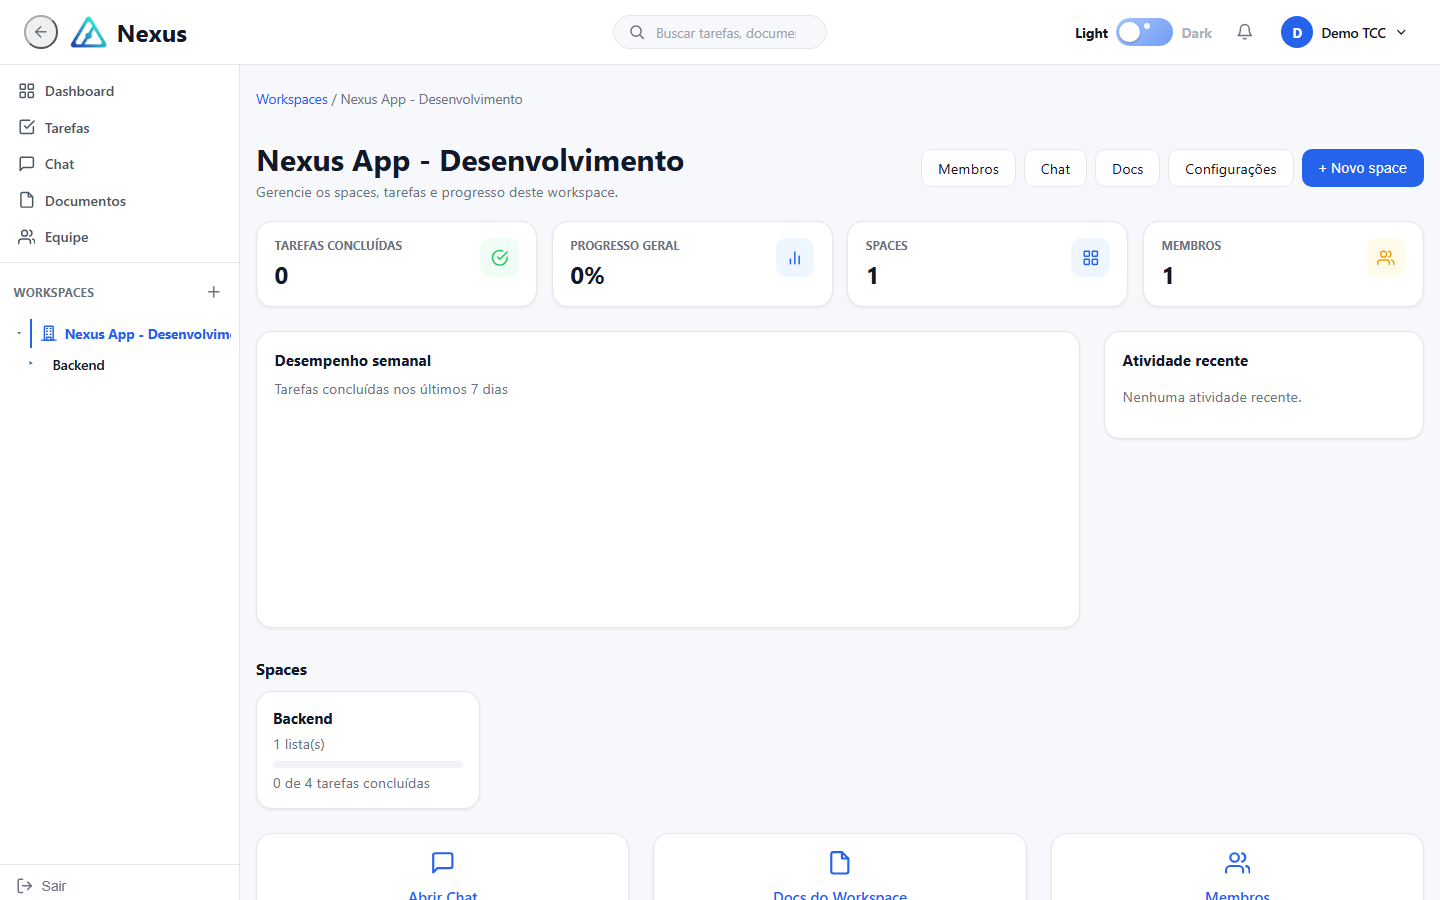
\includegraphics[width=.85\textwidth]{fig-dashboard.png}
\caption{Dashboard de um workspace do Nexus, com KPIs reais, spaces e atividade recente.}
\label{fig:dashboard}
\end{figure}

\begin{figure}[H]
\centering
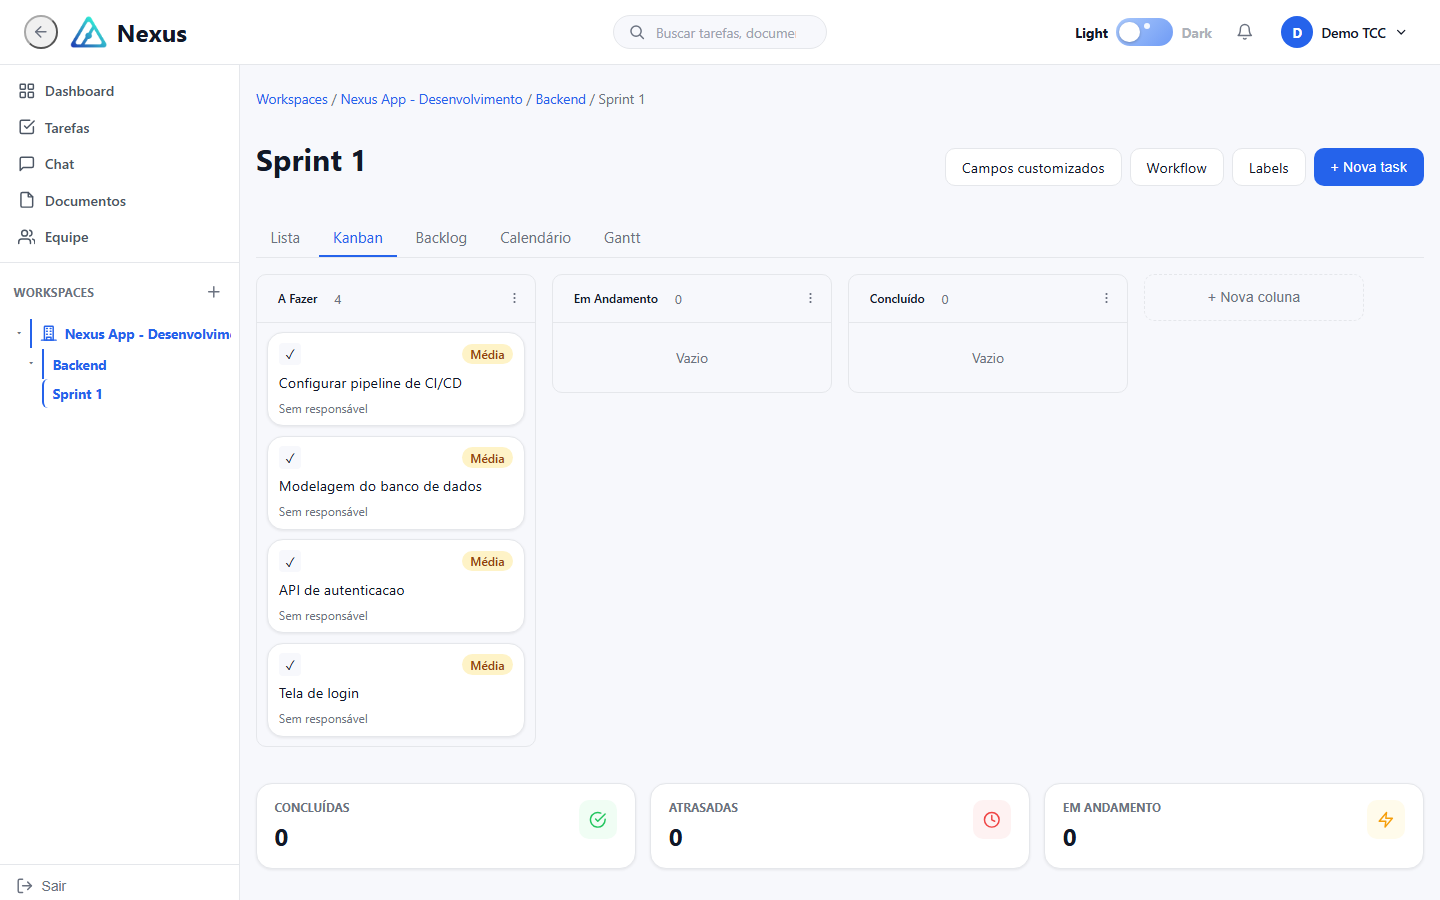
\includegraphics[width=.85\textwidth]{fig-kanban.png}
\caption{Quadro Kanban de uma lista, com colunas configuráveis e tarefas reais criadas via interface.}
\label{fig:kanban}
\end{figure}

\section{Considerações Finais}

O desenvolvimento do Nexus demonstrou ser tecnicamente viável unificar, em um único sistema, funções tradicionalmente oferecidas por ferramentas separadas, sem que essa unificação exigisse abrir mão de especialização de domínio (sprint, burndown, workflow) em favor de um modelo genérico demais para ser útil -- como ocorre na abordagem do Notion -- nem acumular módulos desconexos com curva de aprendizado própria cada um -- como ocorre na abordagem do ClickUp. Os objetivos específicos definidos na Seção~1 foram atendidos: os módulos de gestão de tarefas, documentação e comunicação em tempo real estão implementados e em uso real em produção; o isolamento multi-tenant entre workspaces está implementado via autorização por recurso; e a adequação à LGPD está documentada e implementada, incluindo direito ao esquecimento e portabilidade.

\subsection{Trabalhos Futuros}
\label{sec:trabalhos-futuros}

Dois itens de trabalho futuro concentram a maior complexidade técnica ainda não resolvida no projeto, ambos relacionados à camada de tempo real do sistema.

O primeiro é a \textbf{edição colaborativa em tempo real nas páginas de Docs}. Atualmente, o editor de texto rico é de sessão única: se dois usuários editarem o mesmo documento simultaneamente, a última gravação sobrescreve a anterior sem qualquer resolução de conflito. A proposta é implementar edição simultânea sem perda de dados, no padrão do Google Docs, por meio de um algoritmo de reconciliação de estado distribuído -- CRDT \cite{shapiro2011crdt} ou Operational Transform \cite{ellis1989concurrency} -- que garanta convergência das réplicas mesmo sob latência de rede variável e reconexões, cenário já observado hoje no circuito Blazor Server em produção.

O segundo é a \textbf{escalabilidade horizontal da camada de tempo real}. O broadcast de chat e o limitador de taxa por circuito hoje mantêm estado em memória de um único processo, premissa que se sustenta apenas enquanto o sistema roda em uma única instância. Rodar mais de um servidor exigiria um \emph{backplane} distribuído (por exemplo, Redis) sincronizando circuitos entre instâncias, conciliando a exigência de \emph{sticky sessions} do Blazor Server (o circuito de um usuário precisa permanecer no mesmo servidor durante a sessão) com o fan-out de eventos originados em outro servidor -- incluindo o tratamento de falha parcial, quando um servidor cai e o circuito precisa reconectar em outro nó sem perder contexto.

Complementarmente, identifica-se como trabalho futuro metodológico a implementação de testes de carga formais (por exemplo, com NBomber ou k6), hoje ausentes, para validar quantitativamente o comportamento do sistema sob múltiplos circuitos simultâneos antes e depois da introdução do backplane distribuído.

\subsection{Dificuldades Encontradas}
\label{sec:dificuldades}

A principal classe de dificuldade encontrada durante o desenvolvimento foi a de \textbf{condições de corrida em operações concorrentes}, decorrentes diretamente da arquitetura de estado do Blazor Server e do uso concorrente do sistema por múltiplos membros de um mesmo workspace: foram identificadas e corrigidas, ao longo do projeto, corridas no aceite duplo de convite de workspace, na ordem de envio de um job de notificação de prazo, e na criação/edição concorrente de sprints. A lição prática foi que controle de concorrência otimista (token de concorrência em nível de linha, como o adicionado à tabela de itens de trabalho) precisa ser tratado como requisito desde o desenho do schema, e não adicionado retroativamente apenas onde um bug já foi observado.

Uma segunda dificuldade foi de natureza distinta: \textbf{particularidades de infraestrutura de deploy}, como uma falha de publicação causada por cadeia de certificado incompleta no FTPS e a necessidade de fixar explicitamente a versão do cliente \texttt{postgres} usada no job de backup da pipeline de CI -- problemas que não aparecem em ambiente de desenvolvimento local e só se manifestam no ambiente real de produção, reforçando a importância de um pipeline de CI/CD que valide o processo de deploy de forma automatizada e repetível.

Por fim, a \textbf{segurança} exigiu esforço contínuo e não uma etapa única: o projeto passou por múltiplas rodadas de auditoria, cada uma revelando achados de severidades distintas (de críticos a baixos) em áreas como sanitização de conteúdo, controle de acesso e proteção de segredos -- evidência de que segurança em um sistema multi-tenant com conteúdo gerado por usuário é uma propriedade que precisa ser continuamente verificada, e não algo garantido pela implementação inicial.

\bibliographystyle{fatecbib}
\bibliography{nexus-refs}

\end{document}
